\mode<presentation>
{
  \usetheme{CambridgeUS}
  \usecolortheme{whale}
  \usecolortheme{lily}

  \setbeamercovered{transparent}
  \usefonttheme[onlymath]{serif}
}

\title[\SystemswithTimeDelayShortName] % (optional, use only with long paper titles)
{\course: \SystemswithTimeDelayName\license}

\subtitle
{Lecture \SystemswithTimeDelayNumber} % (optional)

% Delete this, if you do not want the table of contents to pop up at
% the beginning of each subsection:
%\AtBeginSection[]
%{
%  \begin{frame}<beamer>{Outline}
%    \tableofcontents[currentsection,currentsubsection]
%  \end{frame}
%}


% If you wish to uncover everything in a step-wise fashion, uncomment
% the following command:

%\beamerdefaultoverlayspecification{<+->}


\begin{document}

\begin{frame}
  \titlepage
\end{frame}

\mode<article>{
\maketitle
\tableofcontents
}

%\mode<presentation>{
%\begin{frame}{Outline}
%  \tableofcontents
%  % You might wish to add the option [pausesections]
%\end{frame}}
\section{Transfer Function for Time Delay}

Delays occur often in controls systems - there can be delays due to the requirements for computations to occur in a controller, delays in transmitting signals in a control network, or physical delays such as transportation delays in a fluid system. We would like to be able to analyze control systems that contain delays - and we can, as long as we have a transfer function representation for a delay system. This is the subject of this section.

\begin{frame}{Transfer Functions for Delay System}
\begin{center}
What is the transfer function for this linear system?\vspace{.2in}\\<all>
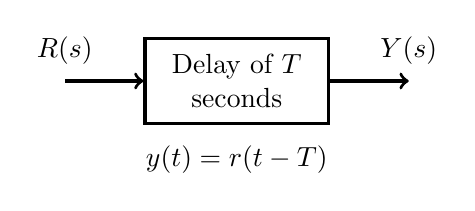
\begin{tikzpicture}[very thick,
sysblock/.style={draw,rectangle,inner sep=6pt,minimum width=1.25cm,minimum height=1.0cm,very thick},
summer/.style={circle,draw,very thick}]

\draw (1.5,0) node[sysblock] (C) {\begin{minipage}{0.75in}\begin{center}Delay of $T$\\ seconds\end{center}\end{minipage}};


%\draw (3.5,0) node[sysblock] (G) {$G(s)$};


\draw[<-] (C.180) -- ++(-1,0) node[above=2pt] {$R(s)$};
\draw[->] (C.0) -- ++(1,0) node[above=2pt] {$Y(s)$};

\draw (1.5,-1) node {$y(t) = r(t-T)$};
\end{tikzpicture}
\end{center}
\end{frame}
To answer the question, we follow the usual steps: Take the Laplace Transform of the defining equation, and find the ratio of the Laplace Transform of the output over the Laplace Transform of the input:
\begin{align*}
\mathcal{L}\{y(t)\} & = \mathcal{L}\{r(t-T)\}\\
Y(s) &= e^{-sT}R(s)\\
 \frac{Y(s)}{R(s)} & = e^{-sT}
\end{align*}
where we used the time delay property to find the Laplace Transform of $r(t-T)$. Thus our answer is, for a delay of $T$ seconds, the Transfer Function is
\[
\boxed{G(s) = e^{-sT}}
\]

Using this and the series connection rules for block diagrams, we can find the transfer function for a system that contains an input or output delay.
\begin{frame}{Systems with Input or Output Delays}
\begin{center}
What are the transfer functions for these linear systems?\vspace{.2in}\\<all>
\input{figures/delay2.tex}
\end{center}
\end{frame}


In both cases, the answer is
\[
\frac{Y(s)}{R(s)} = e^{-sT}G(s)
\]
\section{Frequency Response of Systems with Delays}

What is the frequency response of $e^{-sT}G(s)$?

\begin{itemize}
\item Magnitude Response:
\[
|G(j\omega)e^{-Tj\omega}| = |G(j\omega)||e^{-jT\omega}|
\]
Since $|e^{j\theta}|=1$ for any $\theta$, $|e^{-jT\omega}|=1$, and
\[
|G(j\omega)e^{-Tj\omega}| = |G(j\omega)|.
\]
\begin{quote}
Delay does not change magnitude response.
\end{quote}
\item Phase response:
\[
\angle G(j\omega)e^{-Tj\omega} = \angle G(j\omega) + \angle e^{-jT\omega}
\]
Since $\angle e^{j\theta}=\theta$,
\[
\angle G(j\omega)e^{-Tj\omega} = \angle G(j\omega) - T\omega
\]
\begin{quote}
Phase is shifted by $T\omega$ radians.
\end{quote}
\end{itemize}

\begin{example} Find the Bode plot for the following system with an input delay of 2 seconds.
\begin{frame}
\begin{center}
\input{figures/delay3.tex}
\end{center}
\end{frame}

\begin{itemize}
\item The magnitude response is the same as for $\frac{1}{s+1}$
\begin{frame}
\begin{center}
\includegraphics[width=3in]{figures/example1_1}
\end{center}
\end{frame}

\item The phase response is that of $\frac{1}{s+1}$, but shifted by $-2\omega$ radians. To see the effect of this shift, let's evaluate $-2\omega$ for several frequencies. Note that we will need to convert to degrees when plotting the Bode plot
\begin{center}
\begin{tabular}{ccc}
$\omega$ & $2\omega$ (rad) & $2\omega$ (deg)\\\hline
.01 & .02 & 1.15$^{\circ}$\\
.1 & .2 & 11.5$^{\circ}$\\
.5 & 1 & 57$^{\circ}$\\
1 & 2 & 115$^{\circ}$\\
10 & 20 & 1150$^{\circ}$
\end{tabular}
\end{center}
Note that when $\omega < \frac{1}{T}$, the phase shift is quite small, but when $\omega = \frac{1}{T}$, the phase shift is 1 radian, or $57^{\circ}$, which is substantial, and for $\omega>\frac{1}{T}$ the phase shift is huge. Below, the plot of $\angle \frac{1}{j\omega+1}$ is in green, while $\angle \frac{1}{j\omega+1} - \angle e^{-2j\omega}$ is in blue.
\begin{frame}
\begin{center}
\includegraphics[width=3in]{figures/example1_2}
\end{center}
\end{frame}
\end{itemize}
\end{example}\qed

\begin{example} What is the additional phase lag (in degrees) at $\omega = 5$ rad/s due to a delay of
\begin{itemize}
\item .01 second?
\item .1 second?
\item 1 second?
\end{itemize}


\tryit{
\begin{boxedminipage}{6.5 in}
\rule{0pt}{12pt}\vspace{1in}
\color{lightgray}
\begin{itemize}
\item 2.86$^{\circ}$
\item 28.6$^{\circ}$
\item 286$^{\circ}$
\end{itemize}
\end{boxedminipage}\\
}{\begin{boxedminipage}{6.5in}
For $T=.01$s, 
\[
\omega T= 5 (.01) - .05 \mbox{rad}
\]
converting to degrees
\[
\phi = .05\frac{180}{\pi} = 2.86^{\circ}.
\]
similarly, for $T=1$, $\phi=28.6^{\circ}$ and for $T=10$, $\phi=286^{\circ}$.
\end{boxedminipage}
}

\end{example}\qed



\section{Feedback System Robustness to Delay}


Consider the following system:
\begin{frame}
\begin{center}
\input{figures/delay4.tex}
\end{center}
\end{frame}
\begin{itemize}
\item What delay can be tolerated before the system becomes unstable?
\item Since delay affects phase but not gain, the answer can be found by examining the phase margin.
\end{itemize}

Suppose that $G(s)$ has the following frequency response

\begin{frame}
\begin{center}
\begin{tikzpicture}
\draw (0,0) node {\includegraphics[width=3in]{figures/delaytolerance}};
\draw[thick] (-2.85,2.27) -- (3.1,2.27);
\draw[thick,dashed] (.83,2.27) -- (.83,-2.5);
\draw[<-] (.83,-2.5) -- ++(.5,-.5) node[below right] {$\wco=3$ rad/s};

\end{tikzpicture}
\end{center}
\end{frame}

The phase margin is $\PM=35^{\circ}$, so the delay can make the phase at most $35*\pi/180 = .61$ radians more negative. So how much phase lag does the delay give us? From above, the phase lag in radians is
\[
\phi= \omega T
\]
which depends on frequency. The frequency we should pick is the one where the phase lag is measured. As we know, this is the frequency where the magnitude crosses from above $0$ dB to below $0$ dB, and is called the {\em crossover frequency}, and denoted $\wco$. For this example, the crossover frequency is 3 rad/s. Thus, to find the max delay that can be tolerated before instability, we solve the following equation for $T$:
\begin{align*}
\PM &= \wco{}T\\
.61 &= 3T\\
T &= \frac{.61}{3} = .204
\end{align*}
Note that the units have to be the same on both sides, namely radians, {\em not} degrees.
\section{\textsc{Matlab} Analysis for Systems with Delay}

Here is example \textsc{Matlab} code to plot the Bode plot of a system with an input/output delay.


\noindent\texttt{>> sys=tf([10],[1 1]);\\
>> set(sys,\textquotesingle iodelay\textquotesingle,.164)\\
>> sys\\
\\
Transfer function: \\
\rule{1pt}{0pt}\hspace{1.27in} 10\\
exp(-0.164*s) * -----\\
\rule{1pt}{0pt}\hspace{1.25in} s+1\\
>> bode(sys)}

\begin{center}
\includegraphics[width=3in]{figures/matlabdelay}
\end{center}

\section{Application Example}
\textit{Related to general time delay concepts in the lecture}\\

\noindent We have looked several times at the active prosthetic described in 
\\

\noindent \hangindent=0.5in Samuel Au, Jeff Weber, Hugh Herr, ``Powered Ankle-Foot Prosthesis Improves Walking Metabolic Economy,'' \textit{IEEE Trans. on Robotics}, Vol. 25, No. 1, Feb. 2009.\\

\noindent and in which the following figures appear:

\begin{center}
	\includegraphics[width = 3in]{figures/Prosthetics.png}
	\includegraphics[width = 2in]{figures/Prosthetics2.png}
\end{center}

The authors used frequency response techniques to design the series spring \(k_s\) by plotting the magnitude Bode plot from the maximum input motor force \(F_{sat}\) to the maximum output spring force \(F_s^{max}\), where their goal was to achieve a sufficiently high force bandwidth (see Lecture \TimeFrequencyNumber). In other words, they wanted to achieve a sufficiently high force on the foot plate at high input frequencies.\\


The gain and phase Bode plots for the transfer function \(G(s)\) (without any time delay) given in (Au et al. 2009, p. 57) is shown in Figure \ref{fig:bodePlot}. Notice that both the gain and phase margins are infinite since the gain never exceeds 0 dB and the phase never drops below -180 deg.

\begin{figure}[bh]
\begin{center}
	\includegraphics[width = 4in]{figures/BodePlot.png}\\
	\caption{Bode plot for spring constant design (adapted from Au et al. 2009)}
	\label{fig:bodePlot}
\end{center}
\end{figure}

\textbf{Questions:} If there were a delay of \(T = 1\) seconds in the closed loop system
\begin{center}
	\includegraphics[width = 4in]{figures/ClosedLoopSystem.png}
\end{center}

\begin{enumerate}[(a)]
	\item What would be the gain and phase margins?
	\item How would such a time delay impact the prosthetic user?
\end{enumerate}

\textbf{Answers:} 

\begin{enumerate}[(a)]
	\item The new Bode plot can be created using the \texttt{set(gs,`iodelay',0.1)} command in Matlab (see Lecture \SystemswithTimeDelayNumber) and is shown in Figure \ref{fig:bodePlotWithDelay}.
		\begin{figure}
		\begin{center}
		\includegraphics[width = 4in]{figures/BodePlot2.png}\\
		\caption{Bode plot of $G(s)$ with time delay included. Compare to Figure \ref{fig:bodePlot}.}
		\label{fig:bodePlotWithDelay}
		\end{center}
		\end{figure}
		The time delay causes the phase plot to cross -180 deg at \(\omega_{180} = 23\) rad/s, as shown by the dash-dotted line. The magnitude Bode plot is approximately -3 dB at this frequency, so the time delay causes the gain margin to drop to GM = 3 dB.\\

	\item Additional time delay between the maximum motor force and the maximum spring force could be detrimental to the prosthetic user, even before unstable conditions are reached. Thinking intuitively, the longer it takes for your body to respond, the less well you can expect to perform. 
\end{enumerate}


\section{Lecture Highlights}
The primary takeaways from this article include
\begin{enumerate}
\setlength{\itemsep}{5pt}
\setlength{\parskip}{0pt}
\setlength{\parsep}{0pt}
\item Time delays are common in physical implementations of control systems and must be considered since they can cause closed-loop system instability.
\item When evaluating the impact of a time delay, remember that the delay changes the phase Bode plot but not the magnitude Bode plot. However, both the gain margin and phase margin can be impacted by a time delay since the time delay changes the frequency at which the phase Bode plot crosses $-180^\circ$.
\end{enumerate}

\section{Quiz Yourself}

\subsection{Questions}

\begin{enumerate}
\setlength{\itemsep}{5pt}
\setlength{\parskip}{0pt}
\setlength{\parsep}{0pt}
\item Consider the following feedback system, which contains a time delay. 
\begin{center}
\input{quizfigures/unityfeedback3.tex}
\end{center}
The system $G(s)$ is open loop stable. The Bode plot of $G(s)$ is as follows.
\begin{frame}
\begin{center}
\includegraphics[width=4in]{quizfigures/prob6}
\end{center}
\end{frame}
\begin{enumerate}
\item Find the phase and gain margins if $T_{d}=0$. \vspace{.1in}\\
\item What is the maximum delay $T_{d}$ that can be tolerated before the closed loop system becomes unstable?\vspace{.1in}\\
\end{enumerate}
\end{enumerate}


\subsection{Solutions}
\begin{enumerate}
\setlength{\itemsep}{5pt}
\setlength{\parskip}{0pt}
\setlength{\parsep}{0pt}
\item \rule{12pt}{0pt}
\begin{center}
\includegraphics[width=6in]{quizfigures/1asoln}\\
\end{center}
\end{enumerate}





\end{document}